% Teil Anton

\section{Laver und Benoit: \enquote{Extracting Policy Positions from Political Texts Using Words as Data}  }
In einer Veröffentlichung von Laver und Benoit \cite{LuB} wird eine Methode vorgestellt, bei welcher ohne die Berücksichtigung der semantischen Aussagen eines Textes eine politische Einordnung möglich sein soll, in dem die Wörter als Daten verwendet werden. 
Schon länger ist es ein Anliegen, politische Texte mit objektiven Kriterien in ein gegebenes Spektrum einzuordnen. Verschiede Ansätze beinhalten \enquote{Expert Surveys}, bei welchen die Einschätzungen von Experten herangezogen werden, und \enquote{Crowd Sourcing}, bei welchem die Beurteilungen einer großen Mege Laien verwendet wird. Beide Methoden haben den Nachteil, dass für die Beurteilung einer jeden Quelle ein hoher manueller Arbeitsaufwand nötig ist, um Ergebnisse zu erzielen. \\
Der in  \cite{LuB} vorgestellte Ansatz beschränkt die manuelle Arbeit auf eine konstante Vorleistung, die erbracht werden muss um eine Datenbasis zu generieren und ermöglicht anschließend die vollautomatische Beurteilung von Texten. Die Idee dabei ist, der Häufigkeit wie oft ein bestimmtes Wort in einem Text in Abhängigkeit dessen Länge vorkommt eine Bedeutung beizumessen. 
\begin{itemize}
\item Zunächst werden sogenannte \emph{Reference-Texte} benötigt, deren Einordnung in einer politischen Dimension durch Expert-Surveys oder Crowd-Sourced-Analysis gegeben ist.
\item In jedem der Reference-Texte wird die Häufigkeit aller darin vorkommender Wörter gezählt und durch die Gesamtzahl der Wörter des Textes geteilt, wodruch man die sogenannten Wortfrequenzen erhält.
\item Den Wörtern wird nun in Abhängigkeit ihrer Wortfrequenz eine Beteiligung am Zustandekommen der Ausrichtung des Textes zugesprochen. Wörter mit hoher Frequenz sind in hohem Maße für die Positionierung des Texts verantwortlich, Wörter mit niedriger Frequenz in geringem Maße.
\item Über die Frequenzen der Wörter lässt sich bestimmen, mit welcher Wahrscheinlichkeit man einen bestimmten Text vor sich hat, wenn gegeben ist, dass ein gewisses Wort in ihm enthalten ist.
\item So kann jedem Wort ein sogenannter Word-Score zugesprochen werden. Er sagt aus, wie sehr ein Wort den Text, der es enthält, in eine gewisse Richtung drückt.
\item Nun werden die Wortfrequenzen des zu untersuchenden Texts bestimmt. Dieser Text wird \emph{Virgin-Text} genannt.
\item Mittels der Wortfrequenzen und den zugehörigen Word-Scores kann nun auf eine Position in der zu Beginn festgelegten Skala zurückgerechnet werden, wodurch man eine Einordnung des Virgin-Texts erhält.  
\end{itemize}

\subsection{Berechnungen} \label{Berechnungen}

Konkret werden die folgenden Berechnungen durchgeführt: \\
Seien zu $m\in\N$ die Reference-Texte  $R_1,\ldots,R_M$ und zu $N\in\N$ Virgin-Texte $V_1,\ldots,V_N$ gegeben. 
Mit $a=(a_i)_{i=1}^M\in\R^M$ habe man eine a priori Einordnung der Reference-Texte zur Verfügung.
Das heißt, zu einer festgelegten Dimension $D$ sei $a_i$ die Positionierung von $R_i$, $i=1,\ldots,M$. 
Weiter sei durch $W_1,\ldots,W_K$ mit $K\in\N$ und $W_i\neq W_j$ für $i\neq j$ 
eine Auflistung aller in $R_1,\ldots,R_M$ vorkommenden Wörter gegeben. 
Nun ist die relative Häufigkeit $F_{wr}$ des Wortes $W_w$ in Text $R_r$ durch
\begin{displaymath}
F_{wr} = \frac{|\{W\in R_r:\quad W=W_w  \}|}{|\{W\in R_r\}|}
\end{displaymath}
gegeben. Hieraus erhält man mit
\begin{displaymath}
P_{wr} = \frac{F_{wr}}{\sum_{s=1}^M F_{ws}}
\end{displaymath}
unmittelbar die Laplace'sche Wahrscheinlichkeit beim lesen des Wortes $W_w$ den Text $R_r$ vor sich zu haben. Nun definiert man den Word-Score $S_{w}$ des Wortes $W_w$ auf Dimension $D$ als
\begin{displaymath}
S_w = \sum_{r=1}^M a_r P_{wr}.
\end{displaymath}
Die Positionierungen aller ein Wort enthaltenden Texte fließt also in Abhängigkeit deren Wahrscheinlichkeit in die so gewichtete Positionierung eines jeden Wortes ein, welche dann Score genannt wird. Nun kann mittels dieser Word-Scores die Positionierung der Virgin-Texte berechnet werden. Ist $F_{wv}$ die analog definierte relative Häufigkeit des Wortes $W_w$ im Virgin-Text $V_v$, so kann $V_v$ auf $D$ durch den Score
\begin{displaymath}
S_v = \sum_{w=1}^K F_{wv} S_w
\end{displaymath}
positioniert werden. \\
Die Einordnung der $V_i$ befindet sich aber aufgrund der gemeinsamen Wort-Menge mit allen Reference-Texten auf einer anderen Skala, als die a priorie Einschätzung $a$. 
Daher muss noch eine Normierung durchgeführt werden. Laver und Benoit schlagen folgende Anpassung vor: \\
Sei $\bar{S_v}$ der Mittelwert aller Virgin-Scores und $\Std(S_v),~\Std(a)$ die Standardabweichung der Virgin-Scores bzw. der a priorie Einordnung Reference-Texte. Die normierten Größen $S_v*$ erhält man nun durch
\begin{displaymath}
S_v* = (S_v - \bar{S_v}) \frac{\Std(S_v)}{\Std(a)} +\bar{S_v}. 
\end{displaymath}   
  
  
  \subsection{A priori Ansatz und Induktive Analyse}
Die Autoren unterscheiden zwischen einem \emph{a priori} und einem \emph{a posteriori} oder \emph{induktivem} Ansatz. Während bei ersterem politische Dimensionen als gegeben vorausgesetzt werden und die Reference-Texte dann auf diesen durch Experten oder Laien mit vorher bestehendem Wissen eingeordnet werden, setzt letzter solches Wissen nicht voraus. Im a posteriori Ansatz werden Differenzen der Reference-Texte analysiert, welche dann die Dimensionen bilden, auf denen die Texte entsprechend eingeordnet werden. 
Zur Interpretation der Differenzen wird bestimmten Textpassagen eine Semantik gegeben, welche sich dann in Anzahl und Aussage von anderen unterscheiden kann. Die Autoren kritisieren hierbei, dass in diesem induktiven Ansatzt doch wiederum a priori gegebenes Wissen verwendet wird und entscheiden sich daher direkt den \emph{a priori Ansatzt} zu verwenden.
  
  
  \subsection{Wahl von Reference- und Virgin-Texten}
  Ein bedeutender Schritt ist die sinnvolle Wahl von Refernce- und Virgin-Texten. Mit Begriffen der Linearen Algebra gesprochen, ist es Aufgabe der Reference-Texte den Raum politischer Positionen aufzuspannen, in welchem die Virgin-Texte dann einen Punkt zugewiesen bekommen. Die Refernce-Texte müssen also eine Vektorraumbasis darstellen, die Virgin-Texte müssen Elemente eben dieses Vekotrraums sein. \\
  Laver und Benoit \cite{LuB} geben einige Hinweise, was bei der Wahl von Reference-Texten zu beachten ist. \\
  Zunächst muss für alle in Betracht gezogenen Reference-Texte eine a priori Einordnung auf der Dimension gegeben sein, die untersucht werden soll. \\
  Zweitens sollte der Reference-Text dasselbe Vokabular verwenden wie der Virgin-Text. Daraus ergibt sich, dass rein schriftlich publizierte Texte, wie Parteiprogramme oder Essays wenig geeignet sind, als Referenz für mündlich präsentierte Texte, wie Parlamentsreden oder Talk-Show-Beiträge zu dienen. Auch beim Vergleich von Beiträgen in Medien mit geringerem Anspruch an Formalität, wie soziale Netzwerke, und solchen mit sehr formaler Sprache, zum Beispiel wissenschaftliche Arbeiten, ist Vorsicht geboten. \\
  Drittens sind Reference-Texte damit sie ihre oben erwähnte Basis-Eigenschaft erhalten so zu wählen, dass sie den gesamten Raum politischer Positionen auf gewählter Dimension aufspannen. Haben alle Referenc-Texte ähnliche Positionen zum betrachteten Thema, so sind sie nicht geeignet. Ebenso, wenn ein die gewählte Dimension betreffendes Thema gar nicht behandelt wird.  \\
  Viertens sollten möglichst viele Wörter durch die Reference-Texte auf ihren jeweiligen Word-Score abgebildet werden, damit diese gegebenenfalls zur Bestimmung der Position des Virign-Textes verwendet werden können und damit zufällige Häufigkeiten einzelner Wörter weniger ins Gewicht fallen.  \\
  Diese Überlegungen veranlassen uns, die Texte des Manifesto-Projects als Reference-Texte zu verwenden: Parteiprogramme aller Parteien haben das formale Vokanbular eines schriftlichen Textes, ohne die Fremdwort-Fülle einer wissenschaftlichen Arbeit aufzuweisen. Parteiprogramme sind recht lang und decken alle gesellschaftlich relevanten Theman ab. Durch die kombination von Parteiprogrammen aller demokratischen Parteien sind auch alle demokratischen Positionen vertreten, der gesamte Raum wird aufgespannt. Zuletzt und an wichtigsten: Durch die vorhandene Einordnung der der Texte auf einer Vielzahl politischer Positionen ist es uns erst möglich diese als Referenz zu verwenden. 
  
  
\subsection{Ergebnisse von Laver und Benoit} \label{LuBErgebnisse}
Laver und Benoit \cite{LuB} wenden ihre Methode auf die Wirtschaftspolitik britischer und irischer Parteien an. Dabei verwenden sie Parteiprogramme von 1992 als Reference Texte und Parteiprogramme von 1997 als Virgin-Texte, die sie gleichermaßen von Experten haben beurteilen lassen. In den Abbildungen \ref{fig:Tab2} und \ref{fig:Tab3} sind die Ergebnisse zu sehen. Den fettgedruckten Zahlen ist besondere Aufmerksamkeit zu schenken, sie stellen die durch den Algorithmus gewonnene Einschätzung und den durch Experten gegebenen Score dar. Bei den britischen Parteien ergab sich hier durch den Algorithmus ein Score von $5.0$, $9.71$ bzw. $17.18$ für die Liberale, die Labour bzw. die Konservative Partei; demgegenüber stehen die Einschätzungen der Experten mit $5.77$, $10.3$ bzw. $15.05$ in der gleichen Reihenfolge. Die Übereinstimmung ist augenscheinlich.

\begin{figure}
   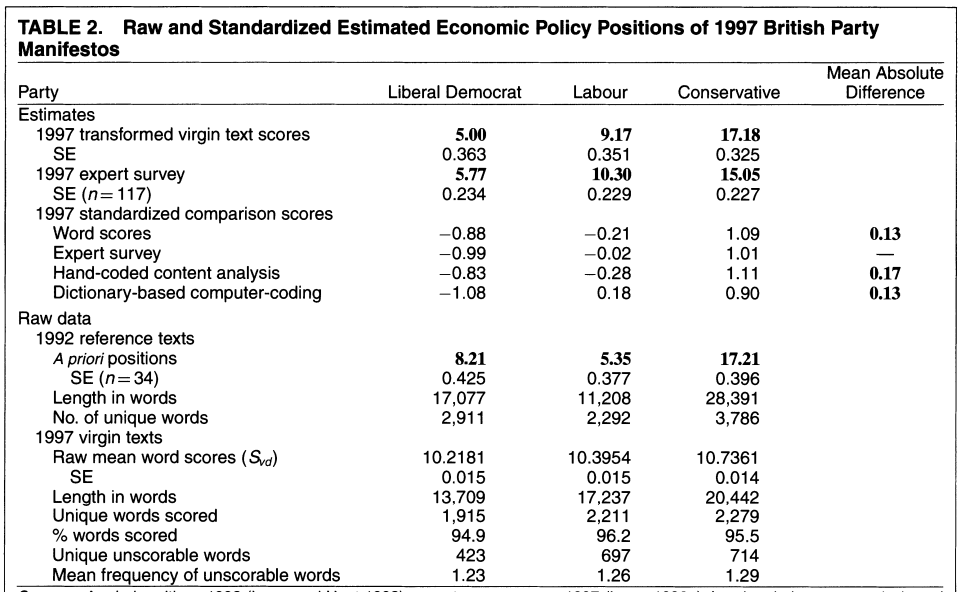
\includegraphics[width=\textwidth]{images/Tab2_LuB.png}
   \caption{Ergebnisse von Laver und Benoit bei Betrachtung der wirtschaflichen Positionenen britischer Parteien \cite{LuB}.\label{fig:Tab2}}
\end{figure}
\begin{figure}
   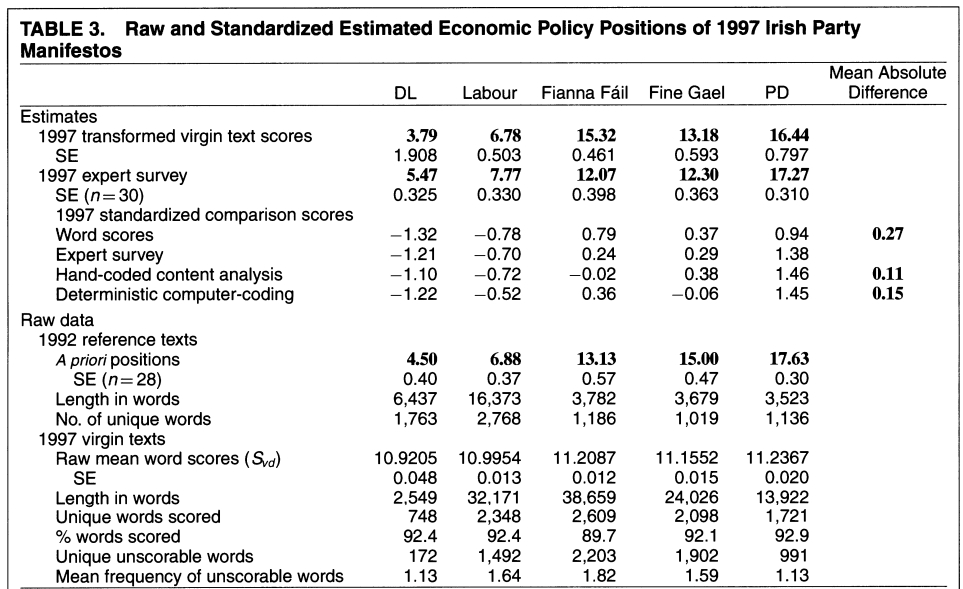
\includegraphics[width=\textwidth]{images/Tab3_LuB.png}
   \caption{Ergebnisse von Laver und Benoit bei Betrachtung der wirtschaflichen Positionenen irischer Parteien \cite{LuB}. \label{fig:Tab3}}
\end{figure}

  
\section{Implementierung in Matlab}
Um die eben erläuterte Vorgehensweise an Anwendungsbeispielen zu untersuchen, ist ein Matlab-Programm geschrieben worden, welches nun vorgestellt werden soll.

\subsection{Funktionen}
\begin{enumerate}[(a)]
\item \label{wordFreq} \texttt{[W, F] = wordFreq( T )} \newline
      INPUT: Cell-Array \texttt{T} mit Texten als Character-Array \newline
      OUTPUT: Cell-Array \texttt{W} mit allen in \texttt{T} vorkommenden Wörtern. \texttt{F} ist eine Matrix, deren Element $f_{ij}$ die relative Häufigkeit des $i$-ten Wortes aus \texttt{W} im $j$-ten Text aus \texttt{T} enthält. 

\item \label{wordScore} \texttt{S = wordScore(F, PP)} \newline
      INPUT: Matrix \texttt{F} aus Funktion (\ref{wordFreq}) und Matrix \texttt{PP} mit \texttt{size(PP,1) == size(F,2)}, welche in Zeile $i$ die politische Positionen des in Spalte $i$ von \texttt{F} bedachten Textes enthält, bezüglich der \texttt{size(PP,2)} zuvor frei gewählten Dimensionen.  \newline
      OUTPUT: Matrix \texttt{S} mit \texttt{size(S,1)==size(F,1)}, \texttt{size(S,2)==size(PP,2)} die in jeder Zeile die Word-Scores zu den entsprechenden Worten und Dimensionen aus \texttt{PP} enthält.
 
   
\item \label{virginScore} \texttt{VS = virginScore(VF, RS)} \newline
      INPUT: Matrizen \texttt{VF} mit den aus Funktion (\ref{wordFreq}) gewonnen relativen Worthäufigkeiten in den Virign-Texten und \texttt{RS} mit den aus Funktion (\ref{wordScore}) gewonnen Word-Scores. \newline
      OUTPUT: Matrix \texttt{VS} mit den Virign-Scores der Texte aus \texttt{VF} bezüglich der mit \texttt{RS} festgelegten Dimensionen.
   
\item \label{transVS} \texttt{PPvir = transVS(PPvir, PPref)} \newline
      INPUT: Matrizen \texttt{PPvir} und \texttt{PPref} deren Zeilen die politischen Positionen der Virgin- bzw. Reference-Texte enthält (erstere gewonnen durch Funktion (\ref{virginScore}), zweitere a priori gegeben). \newline
      OUTPUT: Berechnet die in Abschnitt \ref{Berechnungen} erläuterten normierten Virgin-Scores und gibt die damit aktualisierte Matrix \texttt{PPvir} zurück.
   
\item \label{getStatements} \texttt{[texts, lastname, parid] = getStatements(id)} \newline
    Lädt die Facebook-Statements der Politiker, deren ID im Array \texttt{id} enthalten ist, aus der SQL-Datenbank und gibt diese in \texttt{texts} zurück, zusammen mit deren Nachname in \texttt{lastname} und Partei-ID in \texttt{parid}.

\item \label{getcmpref} \texttt{[reftxt, pp, partyid] = getcmpref(dim, filter, years, party)} \newline
    Lädt als Reference-Texte verwendeten CMP-Texte zusammen mit deren politischer Einordnung und der Partei-ID und gibt diese über die OUTPUT-Variablen \texttt{reftxt}, \texttt{pp} bzw. \texttt{partyid} zurück. Die INPUT-Parameter \texttt{dim} und \texttt{filter} müssen angegeben werden. \texttt{dim} ist hierbei einer der CMP-Dimensionen. Mit \texttt{filter =}\linebreak\texttt{'text'|'filter1'|'filter2'} wird die gewünschte Filterstufe festgelegt. Die Parameter \texttt{years} und \texttt{party} sind optional, mittels Ihnen können die Reference-Texte auf einen bestimmten Zeitraum oder bestimmte Parteien eingeschränkt werden. Bsp.: \texttt{years = [1990 2010]} liefert alle Texte aus dem Zeitraum $1990$ bis $2010$; \texttt{party = [1 2]} liefert nur Texte von CDU und SPD.

\subsection{Skripte}
Die folgenden Skripte wurden vorbereitet. Die berechnen und plotten unter Verwendung der oben aufgelisteten Funktionen die Einordnung verschiedener Texte in zwei Dimensionen, welche aus einer Teilmenge der CMP-Dimensionen gewählt werden können.

\begin{enumerate}
\item \verb|main_lr| \newline
Dieses Skript nimmt eine Simple Links-Rechts-Skala an, auf welcher sechs der sieben größten deutschen Parteien ein Wert zwischen $-1$ (links) und $+1$ (rechts) zugeordnet wird. Die Positionierung der siebten Partei wird dann berechnet. Als Textbasis werden die Parteiprogramme zur Bundestagswahl 2017 verwendet.

\item \verb|main_es|
Als Reference-Texte werden die Texte der Parteiprogramme von 2009 verwendet, als Virgin-Texte die von 2013. Alle Daten werden aus der CMP-Datenbank gewonnen. In einem zweidimensionalen Plot können nun die Platzierungen der früheren Parteiprogramme nach CMP und die berechnete Plazierung der Parteiprogramme von 2013 betrachetet werden. Zu dem werden die CMP-Positionen der Parteiprogramme von 2013 durch $\times$ markiert, wodurch ein Vergleich der berechneten Werte mit den CMP-Werten möglich ist.

\item \verb|main_ms| \newline
Als Reference-Texte werden die Texte des CMP verwendet, deren Einordnung auf gewissen vorgegebenen Skalen ebenfalls druch CMP gegeben sind. Als Virgin Texte werden die Parteiprogramme zur Bundestagswahl 2017 verwendendet. In einem zweidimensionalen Plot können nun die Platzierungen der früheren Parteiprogramme nach CMP und die berechnete Plazierung des diesjährigen Parteiprogramms betrachetet werden.

\item \verb|main_fb| \newline
Die Reference-Texte und wählbaren Dimensionen sind die gleichen wie in \verb|main_cmp|. Als Virgin-Text werden jedoch Facebook-Postings verscheidener Politiker verwendet und deren Einordnung betrachtet. 

\end{enumerate}

   
\end{enumerate}


\section{Anwendung}
Das eben vorgestellte Programm soll nun auf einige aktuelle Beispiele angewandt werden.
    \subsection{Naive Links-Rechts Dimension mit Parteiprogrammen als Text-Basis}
    Zunächst sollen alle derzeit im Bundestag vertretenen Parteien in einem einfachen links-rechts Spektrum eingeordnet mit ihren Parteiprogrammen als Reference-Texte dienen, um dann mit den Parteiprogrammen der beiden ab September höchstwahrscheinlich hinzustoßenden Parteien als Vrigin-Texte, die Position zu der Neulinge zu berechnen. Die Positionen sollen im Intervall $[-1,1]$ repräsentiert werden, wobei $-1$ links und $+1$ rechts bedeutet. Wir schlagen folgende Zuordnung vor:
    \begin{lstlisting}[style=Matlab-editor]
PP = [      0;      % CDU
           -0.25;   % SPD
           -0.5;    % GRN
            0.1;    % CSU
           -0.75    % LKS
      ];    
    \end{lstlisting}
      
     Die auf dieser Referenz-Basis einzuordnenden Parteien sind FDP und AfD. 
     Zunächst werden die relativen Wort-Häufigkeiten in allen Parteiprogrammen berechnet. 
     Mit den Positionierungen der Referenz-Parteien kann damit ein Word-Score für jedes Wort ermittelt werden.
     Diese Word-Scores ergeben Abhängigkeit der Wort-Häufigkeiten in den Virgin-Texten die gesuchte Positionierung:
    \begin{lstlisting}[style=Matlab-editor]
Score FDP  = -0.58553 
Score AfD  =  0.042483
    \end{lstlisting}
    Die FDP befindet sich nach Aussage dieses Modells auf der Link-Rechts-Skala also etwas links der Grünen, die AfD etwa auf Höhe der Union.
    
    
    \subsection{Parteiprogramme auf Basis der CMP-Daten}
    Nun soll eine Einschätzung der politischer Positionen der Parteien von heute auf Basis von CMP-Reference-Texten erfolgen. 
    Zunächst soll eine Szenario ähnlich dem von Laver und Benoit untersucht werden. 
    Dann wird geschaut, an welcher Stelle die Parteien heute im Verhältnis zu ihreren früheren Positionen stehen, in wieweit also ein Wandel der Parteien selbst stattgefunden hat. 
    Als CMP-Dimensionen werden stets das Engagement im Umweltschutz (\verb|environmental_protection|) sowie die gewünschte Regulation der freien Marktwirktschaft (\verb|market_regulation|) gewählt. Da davon ausgegangen wird, dass diese beiden Variablen in Abhängigkeit stehen, wird eine Anordnung der Positionen entlang einer Ursprungsgeraden erwartet: Erhöter Umweltschutz erfordert verstärkt Eingriffe in dei freie Marktwirtschaft; staatliche Eingriffe in die Marktwirktschaft werden oft mit Umweltschutz begründet. Es wird nicht davon ausgegangen, dass gänzlich unabhängige CMP-Variablen gefunden werden können, daher entscheiden wir uns für diese Variablen, deren Abhängigkeit bekannt und abschätzbar ist.
    
    \paragraph{Einschritt-Vorhersage}
    In dieser Untersuchung werden analog zur Vorgehensweise von Laver und Benoit \cite{LuB}, die Parteiprogramme einer Bundestagswahl als Refernce-Text genutzt, um die Parteiprogramme der darauffolgenden Wahl einzuordenen und mit den CMP-Positionierungen zu vergleichen. 
    Wir wählen das Jahr 2009 als Referenz-Jahr und 2013 als zu untersuchendes Jahr. Die Dimensionen werden gewählt wie Eingangs erläutert. Die untersuchten Parteien sind CDU, SPD, FPD und Linke. Das Ergebnis ist in Abbildung \ref{fig:one20092013} zu sehen.
    
    \begin{figure}
    
        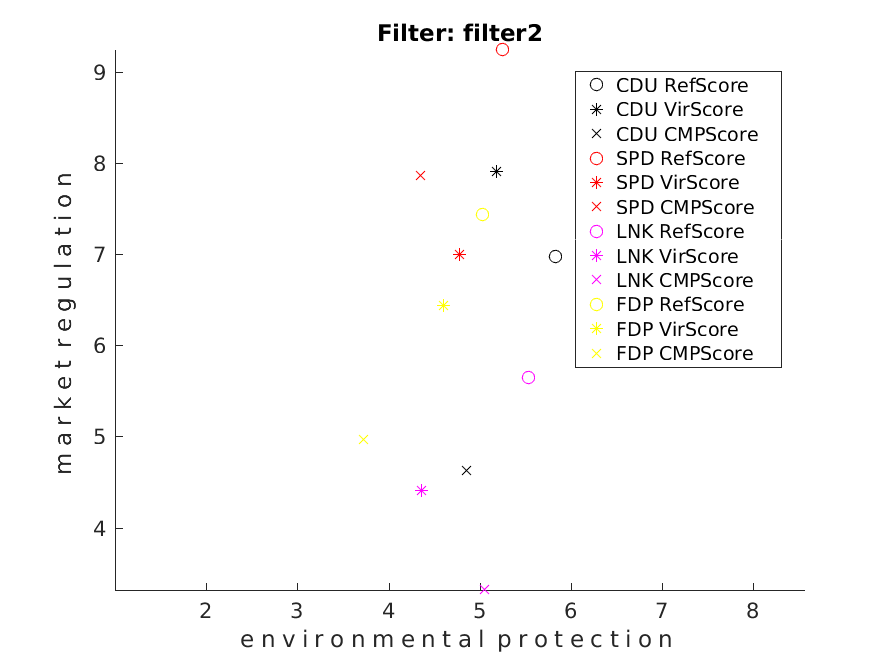
\includegraphics[width = 0.8\textwidth]{images/one_environmental_protection_market_regulation_filter2.png}
        \caption{Einschritt-Vorhersage: Einordnung der Bundestagswahlprogramme von 2013 auf Basis der 2009 und Vergleich mit den CMP-Positionen. 
                 \label{fig:one20092013}}
    \end{figure}
    
Deutlich wird, dass die Ergebisse von Laver und Benoit in dieser Anordnung nicht reproduziert werden können. Ein Zusammenhang der automatischen Einordnung mit der des CMP-Projekts ist nicht zu erkennen.      
    
    \paragraph{Mehrschritt-Vorhersage}
     In diesem Abschnitt werden diesjährigen Parteiprogramme als Virgin-Text gewählt und auf Basis aller in CMP verfügbaren Parteiprogramme seit 1995 beurteilt. Die Texte werden im Originallaut sowie mit beiden Filterstufen verwendet. 
     Die Ergebnisse sind in Abbildung \ref{manifestocmp} zu sehen. Die Häufung entlang der ersten Winkelhalbierenden ist deutlich zu sehen.
     
     
    \begin{figure}
    \centering     %%% not \center
    \subfigure{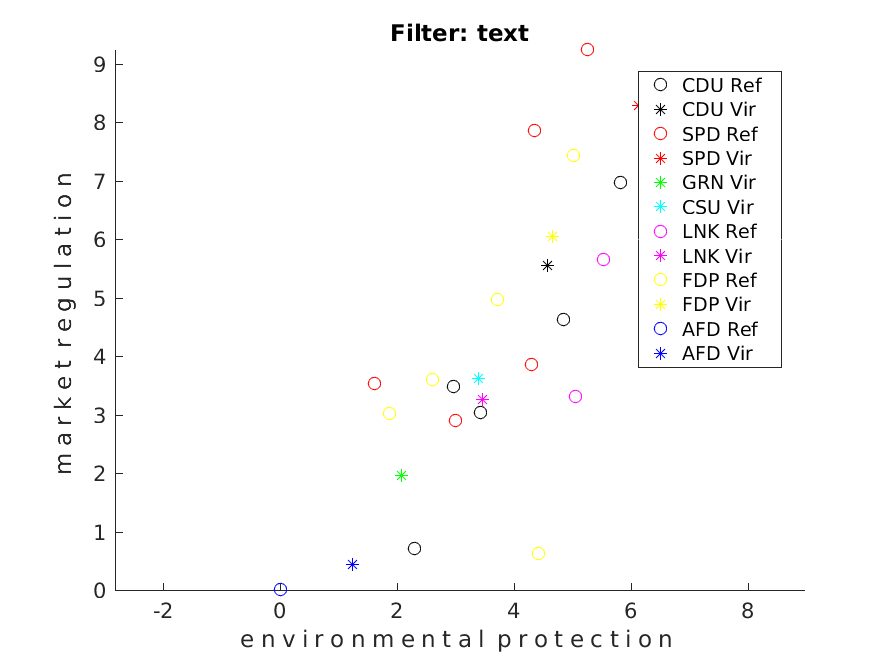
\includegraphics[width=0.49\textwidth]{images/environmental_protection_market_regulation_text.png}}
    \subfigure{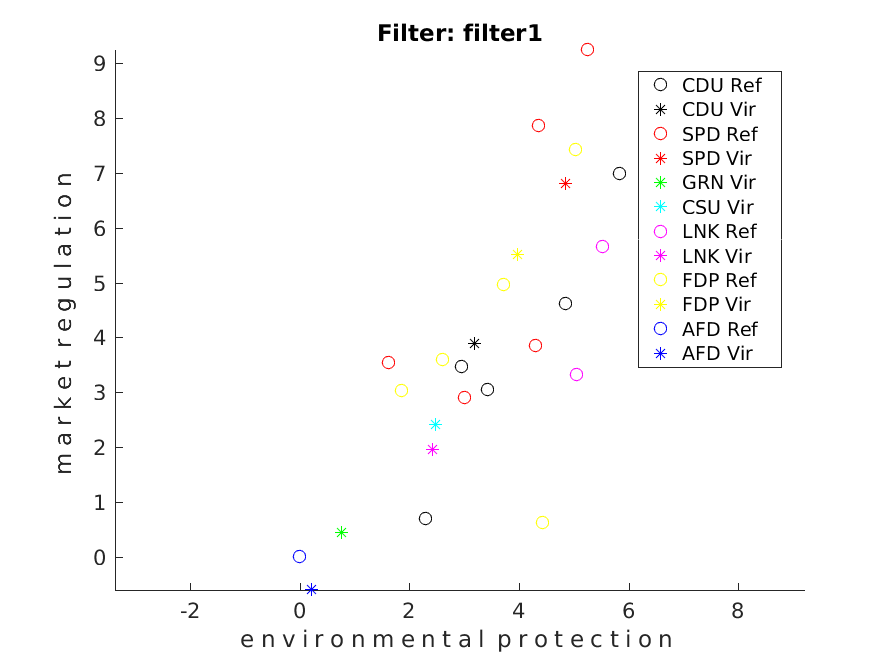
\includegraphics[width=0.49\textwidth]{images/environmental_protection_market_regulation_filter1.png}}
    \subfigure{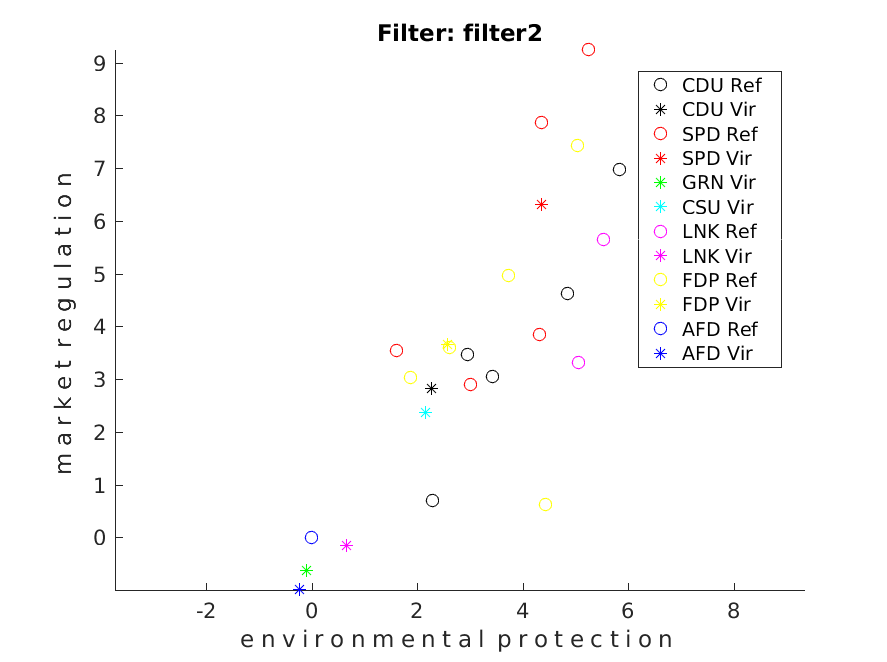
\includegraphics[width=0.8\textwidth]{images/environmental_protection_market_regulation_filter2.png}}
    \caption{Position der diesjähringen Parteiprogramme mit angegebener Dimension und Filter. \label{manifestocmp}}
    \end{figure}
    
    \subsection{Facebookbeiträge auf Basis der CMP-Daten}
    In diesem Abschnitt soll untersucht werden, ob und in wie weit die Aussagen von individuellen Politikern auf Facebook in den Kontext der CMP-Refence-Texte eingeordnet werden können.
     Statt die diesjährigen Partei-Programme als Virgin-Texte zu verweden, werden Beiträge auf den Facebook-Seiten verschiedener Politiker herangezogen. Politische Dimensionen und Reference-Text werden wie im letzten Abschnitt im Paragraph \emph{Mehrschritt-Vorhersage} gewählt. 
     Die Reference-Texte stammen von 1995 bis 2015, die Facebookbeiträge stammen von 2016 und 2017, als Dimensionen wird weiterhin Markregulierung und Umweltschutz gewählt. Da sich die zweite Filterstufe in sofern bewährt hatte, als dass sie den Zusammenhang der beiden Dimensionen an besten wieder gibt, wird der besseren Übersichtlichkeit wegen nur dieser Filter verwendet und auf die anderen Filterstufen verzichtet. Die Ergebnisse sind in Abbildung \ref{fig:fbFilter2} zu finden.
     
     
    \begin{figure}
    
        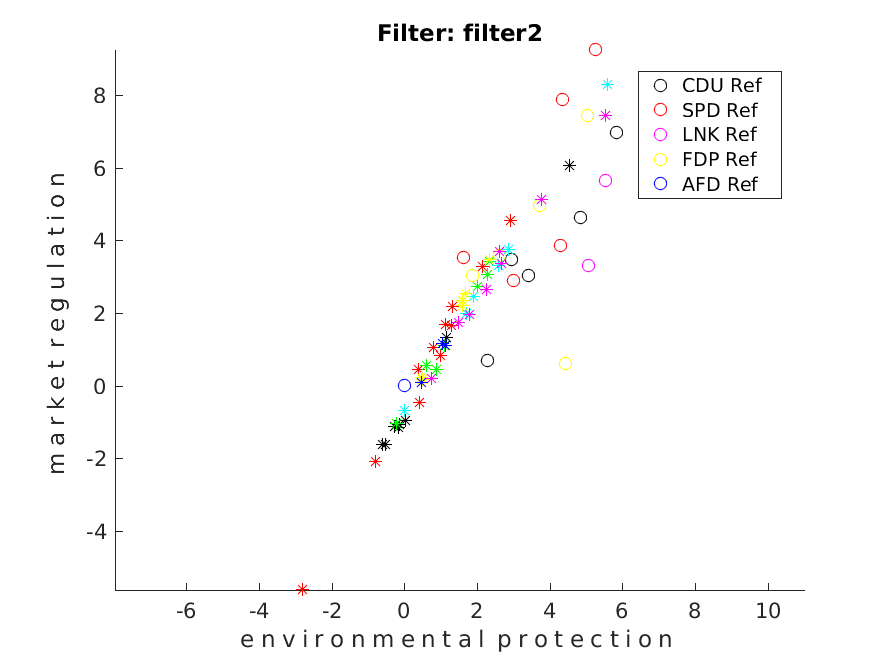
\includegraphics[width = 0.8\textwidth]{images/fb_environmental_protection_market_regulation_filter2.png}
        \caption{Einordnung der Facebook-Beiträge verschiedener Parteipolitiker auf Basis der Bundestagswahlprogramme von 1995 bis 2015. Referenz-Positionen sind durch Kreise markiert, Positionen der Facebookbeiträge werden durch Asterikse dargestellt.
                 \label{fig:fbFilter2}}
    \end{figure}
     
     Während die Abhängigkeit der beiden Dimensionen \verb|market_regulation| und \linebreak\verb|environmental_protection| noch stärker zu Tage tritt, ist eine Zuordnung der Parteipolitiker zu ihren jeweiligen Parteien nicht möglich. Die Verteilung entlang der ersten Winkelhalbierenden mutet an rein zufällig zu sein. Einzig zu beobachten ist, dass die Einordnungen der Facebook-Beiträge insgesamt weniger auf beiden Dimensionen laden, also tendenziell näher am Ursprung liegen. Das kann entweder darauf zurückz zuführen sein, dass auf Facebook weniger deutliche Statements gemacht, bestimmte Buzz-Words, welche auf eindeutige Positionen hindeuten, vermieden und stattdessen lieber allgemeine unverfängliche und positiv klingenden Vormulierungen verwendet werden (\emph{Good Vibes Only}). Es ist aber auch möglich, dass die in Abschnitt \ref{Berechnungen} eingeführte Normierung der Virgin-Scores unzureichend oder für diesen Fall schlicht ungeeignet ist. \\
     Zu beachten ist auch, dass die als Reference-Texte gewählten Parteiprogramme eigentlich nicht geeignet sind um Facebookbeiträge zu untersuchen. Laver und Benoit weißen darauf hin, dass das in Reference- und Virgin-Texten verwendete Vokabular dasselbe sein sollte. Dass diese Bedingung hier erfüllt wird, ist nicht zu erwarten, da in Sozialen-Netzwerken bekanntermaßen eine andere Sprache gesprochen wird, als in offiziellen Partei-Publikationen.
     
    